\documentclass[border=10pt]{standalone}
%%%<
\usepackage{verbatim}
%%%>
\usepackage{pgfplots}
\pgfplotsset{width=7cm,compat=1.10}
\begin{comment}
:Title: Heart in 3D
:Tags: 3D;Color maps;Decorative Drawings
:Author: cmhughes
:Slug: heart-3d

An application of volumes of revolution for plotting
a three-dimensional heart.

This code was written by cmhughes on TeX.SE.
\end{comment}
\pgfplotsset{
  /pgfplots/colormap={pink}{%
    color(0cm) = (purple);
    color(1cm) = (pink!80!purple);
    color(2cm) = (pink!90);
    color(3cm) = (pink) }
}\begin{document}
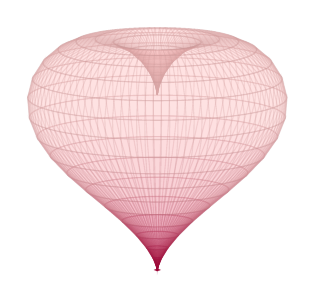
\begin{tikzpicture}
  \begin{axis}[
      view={0}{10},
      axis equal,
      axis lines=none,
      colormap name =pink, 
    ]
    \addplot3[
      surf,
      shader=faceted,
      samples=50,
      domain=0:2*pi,y domain=0:2*pi,
      z buffer=sort,
      opacity=0.15
    ]
    (
      {(sin(deg(x)))^3*cos(deg(y))},
      {(sin(deg(x)))^3*sin(deg(y))},
      {(13*cos(deg(x))-5*cos(2*deg(x))-2*cos(3*deg(x))-cos(4*deg(x)))/16}
    );
  \end{axis}
\end{tikzpicture}
\end{document}
